%****************************************************
%	CHAPTER 1 - INTRODUCTION
%****************************************************
\chapter{Introduction}
\label{ch:intro}
%====================================================
\section{Foreword}
\label{sec:intro.foreword}
%====================================================
\subsection{A Brief Background to the Study}
\label{subsec:intro.foreword.background}
%====================================================
A popular topic for current control and automation research is that of quadrotor UAVs. Attitude control of a quadrotor poses a unique 6-DOF control problem, to be solved with an under-actuated 4-DOF system. As a result the $\phi$ pitch and $\theta$ roll plants aren't controllable. The attitude plant is often simplified around a stable operating point. The trimmed operation region is always at the inertial frames' origin; resulting in a zero-set point tracking problem. The highly coupled non-linear dynamics of a rigid body's translational and angular motions arise from gyroscopic torques [Section:~\ref{subsec:dynamics.nonlinearities.gyrotorques}] and Coriolis accelerations [Section:~\ref{subsec:dynamics.nonlinearities.coriolis}]. These effects are negligible around the origin\footnote{Expanded upon in Appendix:\ref{app:stddynamics}}, hence the origin trim point removes the systems' non-linear complexities. The control system can then reduce each state variable, $\vec{X}_b=\big[\phi~\theta~\psi~x~y~z\big]^T$,to an isolated SISO plant.
\par
As almost every recent quadrotor research paper will mention, the latest interest in the platform is because of recent emergences in availability of MEMS systems and low-cost microprocessors. Such advancements allow for real time state estimation and on-board control loop processing, all at a relatively low cost. Developmental progress in quadrotor and, to a lesser extent, the general UAV field has led to rapidly growing enthusiast community. Companies like HobbyKing\cite{hobbyking} are now synonymous with providing custom made DIY hobbyist quadrotor kits, not just ready to fly commercial products like the DJI Phantom\cite{phantom}.
\par
The avenues for potential application of both fixed wing and VTOL UAVs is expansive, supporting civil\cite{civilquadcopter}, agricultural\cite{agriculturequadcopter} and security\cite{videosurveillancequadcopter} industries. Quadrotor configurations provide a mechanically simple and low cost platform on which to test advanced aerospace control algorithms. Commercial drone use in industry is already a prolific emerging sector; especially in Southern Africa. Subsequently following the $8^{th}$ amendment of civil aviation laws \cite{dronelaw}, use of UAVs for commercial application has now been legalized. Any research into a non-trivial aspect of the field is going to extremely valuable. 
\par
Larger scale quadrotor, hexrotor and even octorotor UAVs are a popular intermediate choice for aerial cinematography due to their high payload capacity.  Whilst still expensive, the cost of a commercial drone like the SteadiDrone Maverik \cite{steadidrone} is far less than chartering a helicopter to achieve the same panoramic aerial scenes or on-site inspections. Another interesting application for UAVs is in the agricultural and cartography surveying sectors. One foreseeable issue which may hinder commercial drone sector progress is the inertial effects associated with large aerial bodies. When scaling up any vehicle, its performance is adversely affected if actuation rates aren't proportionately scaled.
%====================================================
\subsection{Research Questions \& Hypotheses}
\label{subsec:intro.foreword.hypotheses}
%====================================================
The difficulty with control of a quadrotor is that fundamentally it's unstable and under-actuated, \emph{which is empirically proven later with Layupanov Theorem in Chapter:\ref{ch:control}}. The quadrotor has only four controllable inputs, namely propeller rotational speeds $\omega_{1,2,3,4}$ which are then abstracted\footnote{The abstraction of which is explored in Appendix:\ref{app:stddynamics}} to virtual control inputs net torque, $\vec{\tau}_{net}=[\tau_{\phi}~\tau_{\theta}~\tau_{\psi}]^T$, and a perpendicular heave thrust $\vec{T}_{net}=\sum_{i=1}^{4}~T(\omega_i)$. Those four inputs have to affect both the linear X-Y-Z positions and angular pitch, roll and yaw angles, $\vec{\Upsilon}=[\phi~\theta~\psi]^T$. As a result of the under-actuation the attitude control problem becomes a zero set point problem as any other attempt to track attitude cannot be achieved.
\par
The aim of this project is to implement quadrotor attitude and position set point tracking by solving the problem of its inherent under-actuation. Inspired by Boeing/Bell Helicopters' V22 Osprey and the tilting articulation of its propellers, the prototype design proposed here introduces two additional actuators for each of the quadrotors' lift propellers. Specifically, adding rotations about the X and Y axes for each motor/propeller pair. The result is a vectored 3 dimensional thrust force rather than a bound perpendicular lift force. The control problem is then posed as the design of net forces, $\vec{F}_{net} = [F_x\;F_y\;F_z]^T$, and torques, $\vec{\tau}_{net} = [\tau_{\phi}~\tau_{\theta}~\tau_{\psi}]^T$, such that for any given trajectory, $X_d=[x~y~z~\psi~\theta~\phi]^T$, the error state $X_e = X_d - X_b$ asymptotically tends to $\vec{0}$.
\begin{equation} \label{eq:1}
lim_{t \rightarrow \infty} X_e = \vec{0}\hspace{10pt}\forall X \in \mathbb{R}^n
\end{equation}
Where $n$ is the degrees of freedom. The over-actuation brings about the need for a control allocation scheme which distributes the 6 commanded system inputs (net torques and forces) among the actuator set (12 actuators) in order to optimize some objective function secondary to that of Eq:\ref{eq:1}.
\par
Part of the control research question is the multivariable treatment of the system without making any simplifications to the non-linear dynamics involved in the quadrotors motion or making any assumptions about its operational conditions. Standard linearisations applied to the quadrotors' control plant don't hold true for the more aggressive manoeuvres; they're dependent on small angle approximation. Stable control law design will require expansion and simulation of existing kinematic models describing an aerial body and applying them to a quadrotor motion. Thereafter, design, development and control of this new actuator suite which is to be implemented on a quadrotor platform. The final key outcomes for the project are the simulation analysis and prototype construction of the proposed design.
\par
Introducing relative motion within an unconstrained body will produce a lot of unwanted dynamics like inertial and gyroscopic responses, amongst others. A rotating propeller will respond to pitching much like a Control Moment Gyroscope \cite{cmg} or a flywheel. A less trivial result is the aerodynamic torque produced from the propellers' aerofoil profile. Such induced responses occur in planes perpendicular to whatever the propellers' rotation exists in. These aspects are normally canceled out due to a basic quadrotors' co-planar propeller rotation. It's anticipated that a plant dependent control solution will have to compensate for these dynamics, which if left unaccounted for could potentially cause instability. 
%====================================================
\subsection{Significance of Study}
\label{subsec:intro.foreword.significance}
%====================================================
Due to the huge popularity of quadrotor platforms as research tools, any work that improves the UAV \& quadrotor general body of knowledge will prove to be valuable. With that being said, there is already a vast amount of existing research on linear and non-linear control techniques for regular quadrotor platforms. The attitude loop is the most common topic for control research, requiring an under-actuated solution and mostly linearised around the origin (See Appendix:\ref{app:stddynamics}). Far less common is the application of optimal flight path and trajectory planning to quadrotor control. The uniqueness and difficulty of the quadrotor attitude control does not hold true for its position control, so standard techniques can be used for way point planning and the like once the attitude control problem has been answered.
\par
The most significant aspect of this project is the attitude control, discussed later in Section:\ref{sec:control.attitude}. The over-actuation of the proposed design and, more critically, the manner in which the controllers' (virtual) output is distributed among those control effectors would appear to be the first of its kind. Otherwise known as control allocation, the requirements of the distribution algorithm(s) are outlined in Section:\ref{sec:control.allocation}. Dynamic set point attitude control for aerospace vehicles is not a subject heavily researched outside the satellite attitude control field. Even papers which propose similarly complex mechanical over-actuation (expanded upon in next in the literature review, Section:\ref{sec:intro.litreview}) hardly broach the topic of attitude set points away from the origin.
\par
Whilst the control plant (developed in Chapter:\ref{ch:control}) does indeed close both the position and attitude control loops, there is no consideration of trajectory generation nor flight path planning. Such topics are well discussed elsewhere in a far more concise and deliberate way than this project could ever hope to achieve. Once closed loop position and attitude controls have been achieved, the control algorithms can be adjusted to account for higher order state derivative tracking needed for nodal way point planning. The heuristics involved with flight path planning are well documented elsewhere and implementation of them is an academic task.
\par
Where possible the system identification and control (design and allocation) for this project is kept both modular and generically applicable. The intention here is that pertinence falls not only with the UAV field but to any aerospace or free body attitude control. Hopefully the investigation here can be expanded upon with more in-depth research on one of the subsystems without compromising the functionality of the remainder of the whole plant.
\par
Provisionally one possible outcome that the investigation could yield is insight into higher bandwidth actuation and thus a faster control response for larger aerospace bodies. Any standard quadrotor uses differential thrust to develop a torque about its body which suffers a slow inertial deceleration when the propellers change speed. Prioritizing pitching the propellers principle plane of rotation away rather than changes the propellers speed could improve response. This depends on how the allocator block is prioritized (presented in Section:\ref{sec:control.allocation}).
%====================================================
\subsection{Scope and Limitations}
\label{subsec:intro.foreword.scopeandlim}
%====================================================
\subsubsection{Scope}
\label{subsubsec:intro.foreword.scope}
%====================================================
This project includes the conceptualized design and implementation of a novel actuation suite to be used on a quadrotor platform. The express purpose of which is to apply set point attitude tracking control to the body. Stemming from this is an investigation of the associated kinematics which are influenced by the design and its relative motions. In order to apply control theory to achieve the attitude tracking goal, a sound model of the plant dynamics is first needed so that the plants' response can be analysed.
\par
Aspects of the mechanical design are covered in Section \ref{sec:proto.design} but, beyond the cursory investigation, there is no scope for materials analysis or stress testing of the design. To the detriment of the project, the design will either produce an over-engineered or catastrophically under-engineered solution. The focus is rather on the control application and embedded systems design, not the structural integrity of a proposed frame. The only physical measurements made are ones which pertain to the critical kinematics like inertial measurements for the second order gyroscopic and inertial dynamic responses.
\par
As mentioned in the antecedent , Section: \ref{subsec:intro.foreword.significance}, trajectory \& flight path planning are not ubiquitous with this investigation. The kinematic derivation for a 6-DOF body is wholly applicable to any dynamic (rigid or otherwise) aerospace body, although some particular standards are used [sic ZYX Euler Aerospace Sequence, \ref{sec:proto.conventions}]. Similarly the control treatment of the plant is that of a non-linear multivariate control, aided and justified by Lyupanov theorem. Whilst alternative solutions through Model Predictive Control or Quantitative Feedback Theory could provide a more refined or effective controller, they aren't presented and remain open to further investigation. The standard approach for quadrotor attitude control is feedback linearisation of the plant around a trim point to decouple the non-linear dynamics and apply SISO techniques. A derivation of such a linearisation is presented in \ref{app:stddynamics} but there are no further discussions beyond that. Comparison between attitude set point tracking proposed here and normal zero-set point attitude control of fixed rotor quads' is difficult as the fundamental objectives are in stark contrast with each other.
\par
Arguably the most important and indeed novel aspect of this project is the control allocation. Seeing as the system has 12 controllable inputs and 6 possible responses to that input, hence the system is classified as over-actuated. Ergo, there needs to be some logical process as to how those 12 inputs are articulated to achieve the desired 6 movements. Appropriate techniques are first investigated in Section:\ref{sec:control.allocation} and compared before a final solution is implemented in Chapter:\ref{ch:ch5}. It is by no means a comprehensive investigation of every solution possible but rather an analysis of the sub-set of problems and design of what is regarded as a logical and pertinent approach.
\par
With regards to the actual prototype design, in Section \ref{sec:proto.design}, it's assumed that certain aspects are a given certainty. Particularly the state estimation, updated through a 4-camera positioning system fused with a 6-axis IMU through Kalman Filtering, is assumed to precise and readily disposable at a consistent 50 Hz. Hence state estimation is presented but is bereft of intricate detail, this is another topic which has been well documented elsewhere.
%====================================================
\subsubsection{Limitations}
\label{subsubsec:intro.foreword.limits}
%====================================================
By far the biggest constraint of the design is the net weight of the assembled frame. The lift required to keep the body aloft is obviously dependent on the all up weight. Thrust forces disposable to the controller then need to be such that there is clear headroom below actuator saturation during hover flight. The controller effort increases with the magnitude of change for desired state, so steady state actuation conditions must be just a fraction of the maximum actuator outputs. Conversely the all up weight is mostly dependent on the lift motors, being the heaviest part of the vehicle, and their associated power electronics. A trade-off between these two factors makes designing the prototype a balancing act of compromise; added actuation is needed to produce the desired thrust vectoring. That added actuation is going to increase the weight which then requires more thrust force to ensure the vehicle remains airborne. Bigger motors then need stronger actuators to effect the relative motion and overcome the bodies inertial response. It's a compromise between the weight of the body and the strength/quality of the actuation.
\par
To forego the deliberation detailed above, a self imposed limitation applied to the design is to only make use of a particular predetermined motor, namely a set of four Turnigy DST-700 motors. The \dept ~at \uni ~has a surplus of these from previous projects so it saves on new motor costs. A direct consequence of this decision is that the net thrust disposable for actuation is limited to around 700g, $\approx$ 6.9 N, per motor (see Section: \ref{subsec:dynamics.aero.bem}, later in Chapter \ref{ch:dynamics}). This means that all other aspects of the prototype need to adhere to this weight limitation. It is crucial to ensure the control algorithm doesn't induce over-saturation of the motor actuations, so the frame weight needs to be around 40-50\% of the maximum available thrust. These saturation conditions are expanded upon later in Section: \ref{sec:control.allocation} in more detail.
\par
Another aspect of the design limitations resulting from decisions taken, mainly to reduce the costs of construction and complexity, is the use of 180\textdegree ~rotatable servos. The servos are for the individual motors' pitch and roll actuation and act in lieu of continuous rotation DC (brushless or stepper) motors. Any rotation beyond 360\textdegree would require both closed loop position control of the actuator, unlike a servo, and slip rings for power transmission so that no wiring would impede the bodies relative rotation. However the logistics of implementing such a design whilst maintaining an acceptable weight is almost impossible without dramatically scaling up the size of the prototype to accommodate for weight increases.
Commercial camera stabilizing gimbals already make use of similar configurations but the I/O requirements from the flight controller $\mu$C already constricts the amount of expansion at hand.
\par
Some of the discretionary elements for  the whole system will limit performance but are mitigated where possible. For example analogue servos have an associated 1 ms deadband from their 20 Hz refresh rate which can be addressed by using faster, albeit more expensive, digital servos which sample at 333 Hz. The on-board flight control system, see \ref{sec:proto.layout}, needs to apply PWM outputs to 12 different actuators as well as receiving command updates from a ground control station so the I/O capability of most embedded systems are going to be at capacity. Sub-systems will have to be divided and relative inter-communications adopted for various comms and on-board data logging. All of these things are addressed in the following Chapter \ref{ch:proto}.
%====================================================
\section{Literature Review}
\label{sec:intro.litreview}
%====================================================
\subsection{Existing \& Related Work}
\label{subsec:intro.lit.related}
%====================================================
The field of transformable aerospace frames is not necessarily a new one, with many commercial examples having seen a lot of success over their operational life span. The most notable tilting-rotor application is that of the Boeing/Bell V22 Osprey aircraft. First introduced in the field in 2007, the Osprey has the ability to pitch its two lift propellers forward to aid in translational flight after a VTOL manoeuvre has been completed. In addition to this there have been a handful of papers published on similar tilting bi-rotor UAVs' (Fig: \ref{fig:dualaxistilt}\footnote{Image used from G. Gress: \cite{gres2007}}) for research purposes.
\begin{figure}[hbtp]
\centering
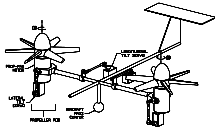
\includegraphics[width=0.7\textwidth]{figs/dualaxistilt}
\caption{General Structure for Opposed Tilting Platform}
\label{fig:dualaxistilt}
\end{figure}
\subsubsection*{Birotors}
Research into birotor vehicles (Fig: \ref{fig:dualaxistilt}) with ancilliary lift propeller actuation is often termed Opposed Active Tilting, \emph{OAT}. Such a rotorcrafts' mechanical design applies either a single \emph{oblique} 45\textdegree ~tilting axis relative to the body; \cite{smalltwotilting,obliquepitch,passiveobliquetilting}, or a \emph{lateral} tilting axis, adjacent to the body; \cite{tiltrotorUAV,adaptivebackstep,tiltrotorcontrol,tpheonix}. Leading research is currently focussed on applying doubly actuated tilting axes to birotor UAVs. Dual axis Opposed Active Tilting or \emph{dOAT} introduces vectored thrust with propeller pitch and roll motions to further expand the actuation suite, \cite{gres2007,opposedlateraldualaxis}. A birotor is sometimes considered preferable to the multirotor platform due to its reduced controller effort. However the controller plant abstraction often detracts from the quality and effectiveness of its treatment as a result of its' underactuation. 
\par
Birotor attitude control incorporates the typical plant independent PD \cite{obliquepitch} and PID \cite{tiltrotorUAV} controller schemes but often more computationally exhaustive and plant dependent Ideal and Adaptive backstepping controllers are investigated, presented in \cite{smalltwotilting,tpheonix} and \cite{adaptivebackstep} respectively. The coupling of a birotor vehicles' attitude system is more prominent than a quadrotors', derived in Section: \ref{sec:dynamics.nonlinearities}, and so feedback linearisation is almost always used. In an interesting progression from the norm, Lee et al,  \cite{autopilotPSO}, proposed a PID co-efficient selection algorithm using a Particle Swarm Optimization techinque, similar to \cite{adaptivepso}. However their performance metric criterion was a basic ITAE term and not anything more unique involving effects specific to flight. \emph{PSO} algorithms iteratively search for a globally optimized solution and offer independent, derivative free optimization. This project report also exploits PSO optimization for non-linear controller coefficient selection, shown in Section:\ref{sec:control.tuning}.
\par
\subsubsection*{Quadrotors}
Expanding on multirotor vehicles, the quadrotor UAV is a popular and well covered research platform due to its relative mechanical simplicity. What would appear to be one of the first quadrotor research implementations, in 2002, is the X4-Flyer quadrotor helicopter, \cite{x4flyer,x4flyercontrol}. Subsequently alternative iterations like the Microraptor, \cite{microraptor}, and STARMAC, \cite{starmac}, quadcopters have been built and tested. A plethora of literature exists around basic quadrotor kinematics \& control \cite{dynamicmodelling2013, dynamicmodelling2009, modelingquadcopter, quaddynamics, fullquadcoptercontrol}, however dedicated 6-DOF rigid body dynamic papers \cite{rigidbodylecture,eulerrigidbody} provide better insight into the appropriate kinematics. Often the dynamics are simplified around a trim point and thus assumed to decompose into 6 SISO plants for each degree of freedom, see Section: \ref{sec:dynamics.rigidbody} and Appendix: \ref{app:stddynamics}. More recent research projects have incorporated advanced aerodynamic effects like drag and propeller blade-element momentum theory into the dynamics; \cite{lowreynolds,bem,starmac}. Although commonly neglected due to their inconsequence under standard opperating conditions, the higher fidelity models are more precise without trim point linearisations \& better modelled thrust calculations; \cite{nonlineardynamics,starmac}.
\par
\begin{figure}[htbp]
\centering
\begin{subfigure}{.5\textwidth}
\centering
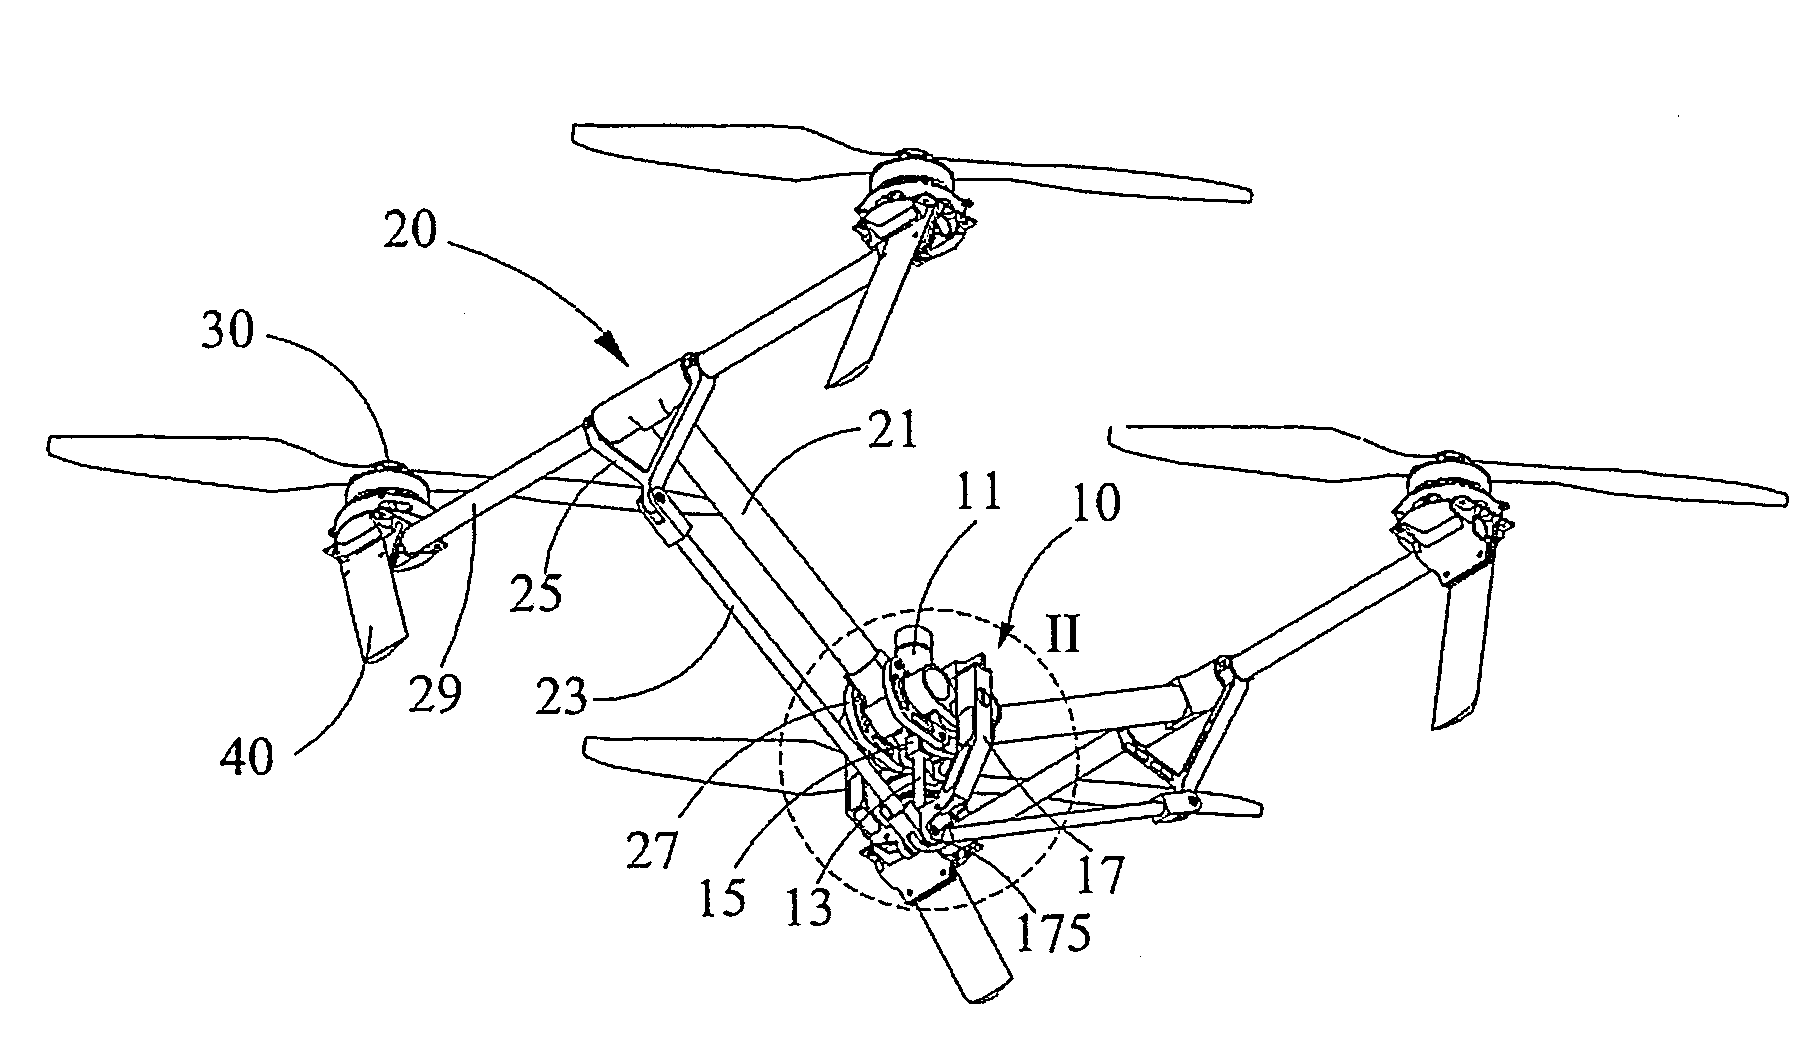
\includegraphics[width=\textwidth]{figs/dji-inspire1}
\caption{Inspire 1 articulated upwards}
\label{fig:inspireup}
\end{subfigure}%
\begin{subfigure}{.5\textwidth}
\centering
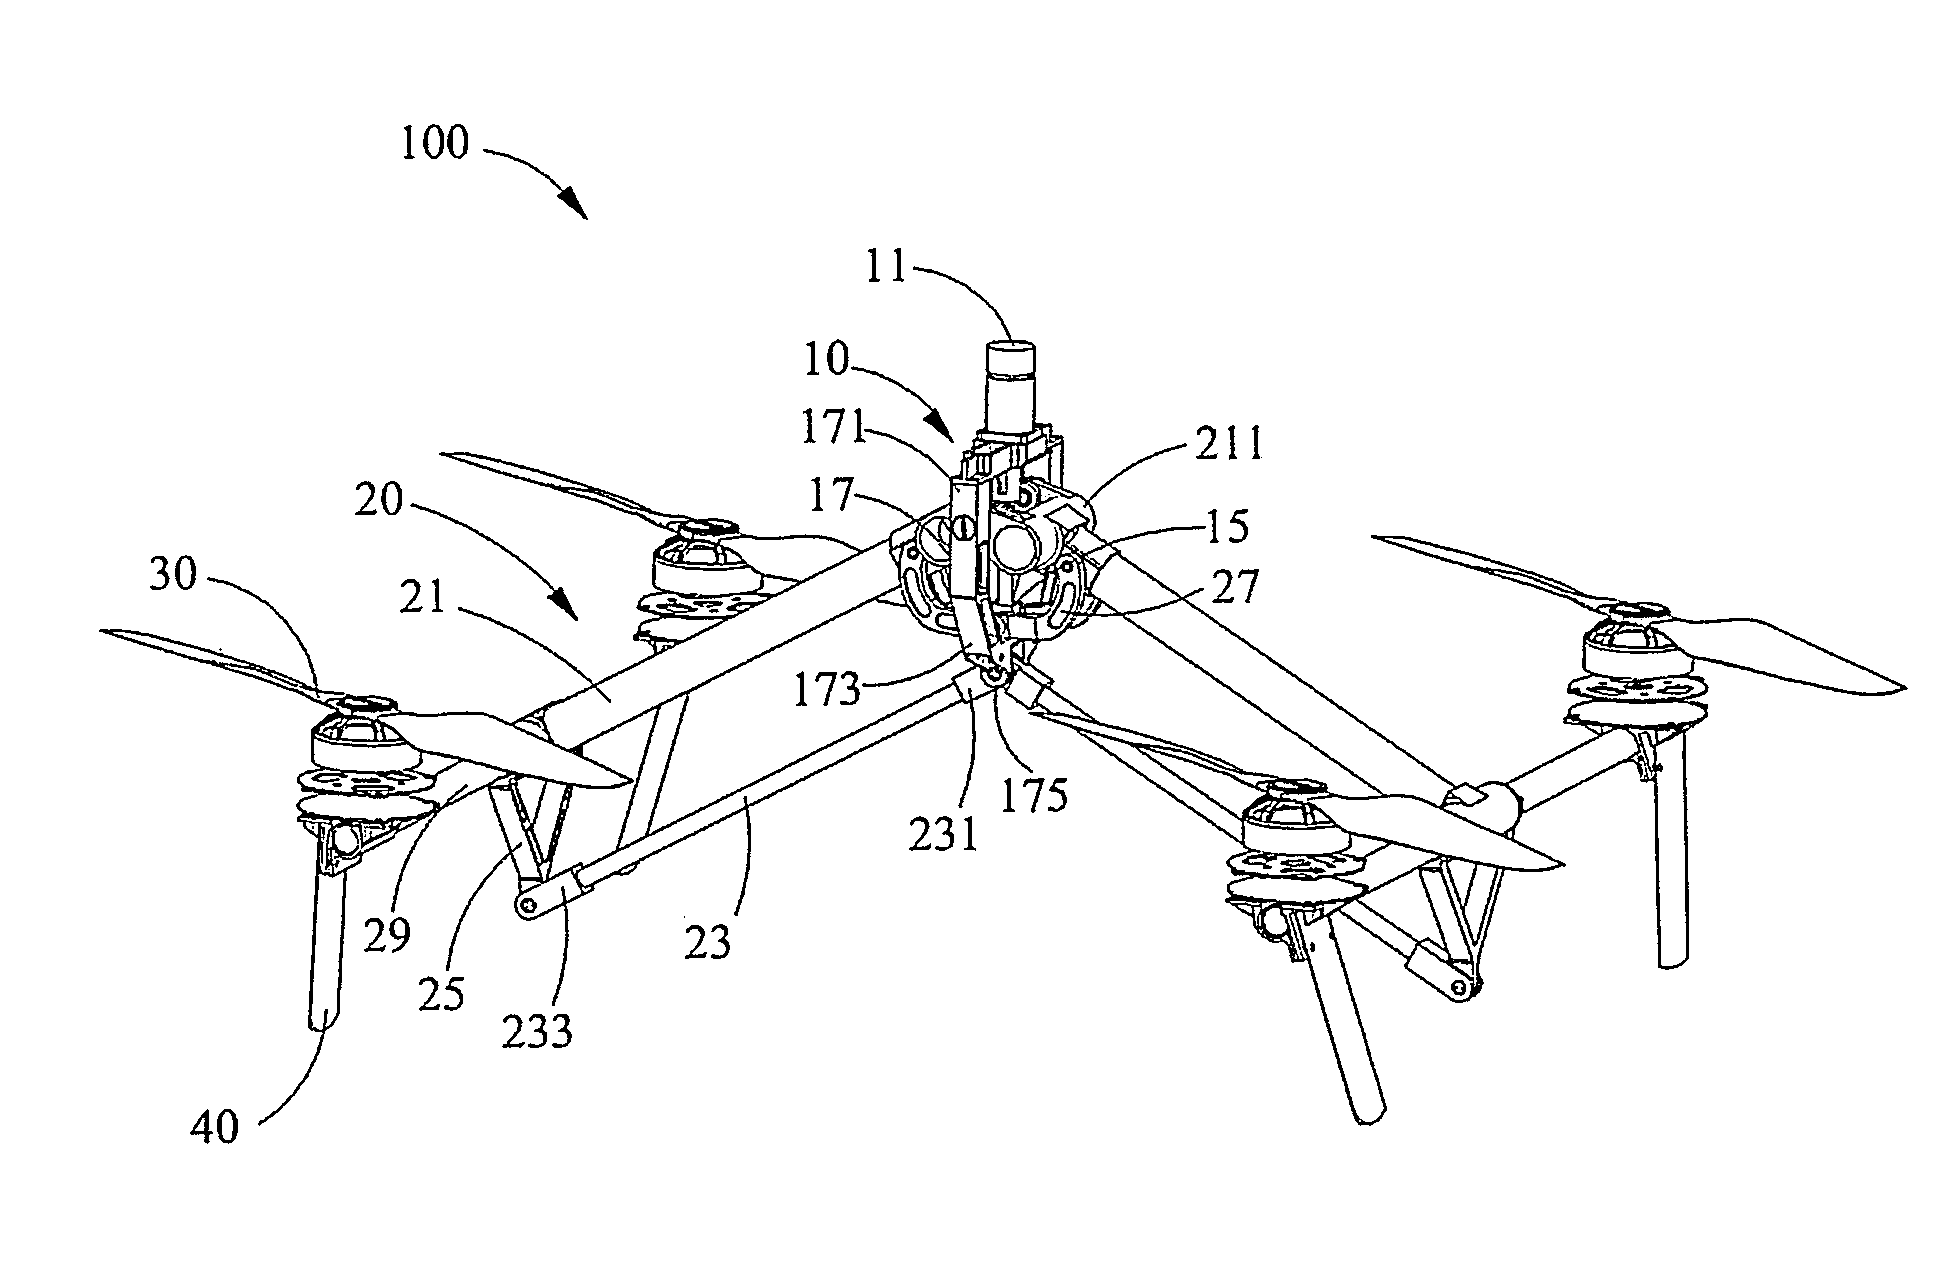
\includegraphics[width=\textwidth]{figs/dji-inspire2}
\caption{Inspire 1 articulated downwards}
\label{fig:inspiredown}
\end{subfigure}
\caption{DJI Inspire 1}
\label{fig:inspire1}
\end{figure}
The only commercial example of a transforming quadrotor is the DJI Inspire1 \cite{inspire}, made by Shenzen DJI Technologies (who are more commonly known for the popular DJI Phantom drone). The Inspire can articulate its supporting arms up and down as shown in Fig:\ref{fig:inspire1} \footnote{Both images were sourced from the drones' patent, held by SZ DJI Tech Co\cite{djinspire}}. The purpose of such movements is to both alter the center of gravity and further expose a belly mounted camera gimbal to achieve panoramic sequences. This transformation changes the moment of inertia about the bodies center of gravity which then changes the inertial torque response induced by angular movements, an otherwise detrimental effect which makes researchers apprehensive of transformable aerospace frames. The range of "transformation" the frame can undergo is just limited to articulating the arms up and down.
\par
In a similar fashion to the progression seen in birotor state-of-the-art, quadrotor research is broaching the topic of single and dual axis tilting articulation. The concept was first conceptualized and implemented on a prototype related to an ongoing project covered in two reports, \cite{tiltpropellercontrol,tiltpropellerflight}. The authors M. Ryll et al.(2012, 2013) modified and tested a QuadroXL four rotor helicopter, propduced by MikroKopter \cite{mikrokopter}, to actuate a single axis of tilt aligned with the frames arms (Fig:\ref{fig:tiltpropellercontrol1}\footnote{Image sourced from Modelling and Control of a Quadrotor UAV with tilting propellers, \cite{tiltpropellercontrol}}). Their proposed control solution, discussed in detail next in Sub-section:\ref{subsec:intro.lit.control}, assumes no nominal linearised conditions around hover flight unlike a similar single axis tilting quadrotor prototype designed by Nemati, et al. (2012)\cite{singleaxistilting}. The latter remains  \underline{simulated} but as yet untested.
\begin{figure}[htbp]
\centering
\begin{subfigure}{.5\textwidth}
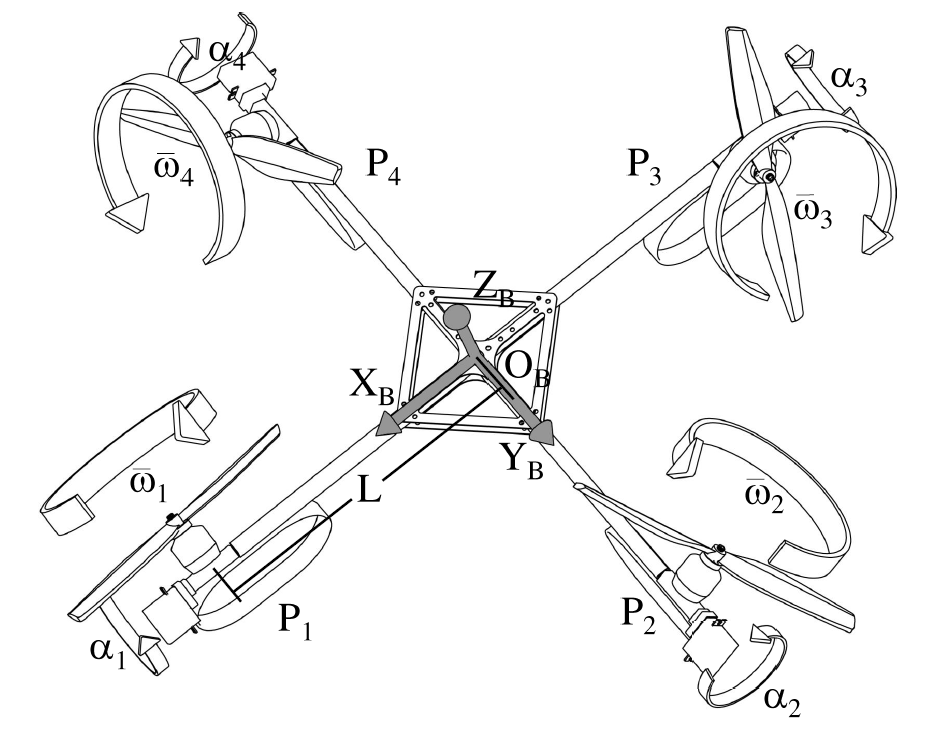
\includegraphics[width=\textwidth]{figs/tiltpropellercontrol1}
\caption{Single rotation axis aligned with the frames arm}
\label{fig:tiltpropellercontrol1}
\end{subfigure}%
\begin{subfigure}{.5\textwidth}
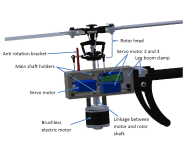
\includegraphics[width=\textwidth]{figs/napsholm-mech}
\caption{Cyclic-pitch \& swashplate mechanism}
\label{fig:tiltrotor-napsholm}
\end{subfigure}
\caption{}
\label{fig:tiltprop}
\end{figure}
\\
One approach to improving quadrotor flight operation is to alter the manner in which the thrust is actuated. Drawing from helicopter technology, a paper by Napsholm, (2013)\cite{napsholm}, has designed a prototype quadrotor UAV which uses co-axial swashplates for varying the propeller pitch. His aim was a design which didn't rely power electronics to change the BLDC motors' speed for thrust actuation, hoping to eventually replace the BLDC motors with petrol combustion engines. Furthermore, the design applied a single axis of tilting actuation to each of the four motor modules. Whilst mechanically complex, Napsholm made use of existing RC helicopter components to design a rotor actuation bracket (Fig:\ref{fig:tiltrotor-napsholm}). The cyclic-pitch swashplate actuation \cite{autonomousrobotspitch} can apply pitching and roll torques, $\tau_{\phi}$ and $\tau_{\theta}$, about the propellers' \emph{principle axis of rotation}. The bandwidth of such an actuator is far greater than that of a differential torque produced rolling/pitching motion.
\par
Regardless of his strong initial theoretical grounding in the early stages of his project, it would appear that Napsholms research suffered due to time constraints. The introductory derivation on aero-dynamical effects and deliberation over the design provide clear insight into the projects goals. However the control solution and system architecture, electronic and software, are left wanting. An introductory proposal of an MPC attitude control system detracted from the comprehensive dynamics discussed. The project obviously ended before testing, simulation and results could be achieved. Unfortunately, despite the novel and over-actuated design, there was no discussion given on how the allocation would be performed.
\par
Finally, the most crucial research to mention is that of a project completed by Pau Segui Gasco \cite{tiltgasco}, which was a dual presented MSc project with Yazan Al-Rihani \cite{tiltrihani}. At the time of writing, this would appear to be the only project published pertaining to \emph{over-actuation} in aerospace bodies implemented on a quadrotor platform. The research was split between the two authors who completed the control/electronic design and the mechanical platform design for their respective dissertations. Shown in Fig:\ref{fig:tiltrotor-gasco}\footnote{Development of a Dual Axis Tilt Rotorcraft UAV: Modelling, Simulation and Control \cite{tiltgasco}}, the dual-axis articulation is achieved using an RC helicopter tail bracket and push-rod mechanism; reducing the mass of the articulated component but limiting the range of actuation. Considering the spinning propellers and their induced gyroscopic torque as an actuator plant, the commanded virtual control is then distributed by weighted inversion amongst the actuator set. The whole projects justifies the extra actuation as redundancy but doesn't necessarily prove how such a redundancy could be beneficial.
\begin{figure}[htbp]
\centering
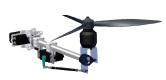
\includegraphics[width=0.7\textwidth]{figs/gasco-mech}
\caption{Dual-axis tilt-rotor mechanism}
\label{fig:tiltrotor-gasco}
\end{figure}
%====================================================
\subsection{Notable Quadrotor Control Implementations}
\label{subsec:intro.lit.control}
%====================================================
\subsubsection*{Quadcopter Attitude Control}
%====================================================
Attitude control of a 6-DOF body is a well understood topic, best described by \emph{The Attitude Control Problem} \cite{attitudecontrolproblem}, whereby a rigid body currently has an attitude state $E_s$ and a desired state $E_d$. The problem is to then find a torque control law:
\begin{equation} \label{eq:2}
\tau = f(E_s,E_d,\omega_s,\omega_d)
\end{equation}
Such that $lim_{t\rightarrow\infty}E_s \rightarrow E_d$ asymptotically as $t \rightarrow 0$ and $\omega_s \rightarrow \omega_d$ similarly. Depending on how the attitude is posed; with rotation matrices \cite{rigidbodylecture,eulerrigidbody,rotationsequences}, quaternions \cite{quaterniondynamics, rotationsequences, spacecraftattitutdequaternions,fullquaternion} or otherwise (Direct Cosine Matrix etc \ldots) the dependent error sate $E$\footnote{\emph{The Attitude Control} \cite{attitudecontrolproblem} describes these conventionally different error states}$= E_d - E_s$ could then differ. Simulation and modelling papers often rely on Euler angle based rotation matrices for attitude representation, \cite{quadsimulationcontrol, adaptivedisturbancecontrol, optimizedpidquadcopter, singleaxistilting, backsteppingquadcoptercontrol, fullquadcoptercontrol} without addressing the inherent singularity associated with such an attitude representation [sic Gimbal Lock, \cite{euleranglesingularity}, Section:\ref{subsec:dynamics.rigidbody.singularity}]. The alternative quaternion attitude representation, first implemented on a quadrotor UAV in 2006 \cite{attitudestabilization}, often used in lieu of rotation matrices has its own caveat of \emph{unwinding}, (Section:\ref{subsec:dynamics.rigidbody.unwinding}), as a result of quaternions dual-coverage \cite{unwinding}.
\par
Quadrotor plant dynamics, as mentioned before, are often linearised; especially when represented with a 3-variable Euler angle set, $E = [\phi ~\theta ~\psi]^T$. The coupled gyroscopic and Coriolis responses are both neglected when the angular velocity rate is small, $\vec{\Omega} \approx 0$, and the inertial matrix is diagonal, $rk(\mathbb{I}_b)= x$ for $\in\mathbb{R}^x$. The consequence of which is the ineffectual deterioration of both the gyroscopic term, $\tau_{gyro}=\vec{\Omega} \times \mathbb{I}_b\vec{\Omega} \approx 0$ and the  Coriolis force term, $F_{cor}=-\vec{\Omega} \times \vec{a_b} \approx 0$ in the bodies dynamics~[Chapter:\ref{ch:dynamics} for context]. Once the cross-product coupled terms are no longer of consequence, each of the 6 degrees of freedom, $[X ~Y ~Z]^T, [\phi ~\theta ~\psi]^T$, can be treated as an individual SISO plant with appropriate techniques used. Quaternion represented attitude plants cannot easily be decomposed into individual SISO controllable plants [Quaternion dynamics in Section:\ref{subsec:dynamics.rigidbody.quaternion}]. So a quaternion (combined four variable attitude state vector) is then used, $Q_b = [q_0 ~\vec{q}\>]^T$ for the abstracted major loop plant.
\par
\begin{figure}[hbtp]
\centering
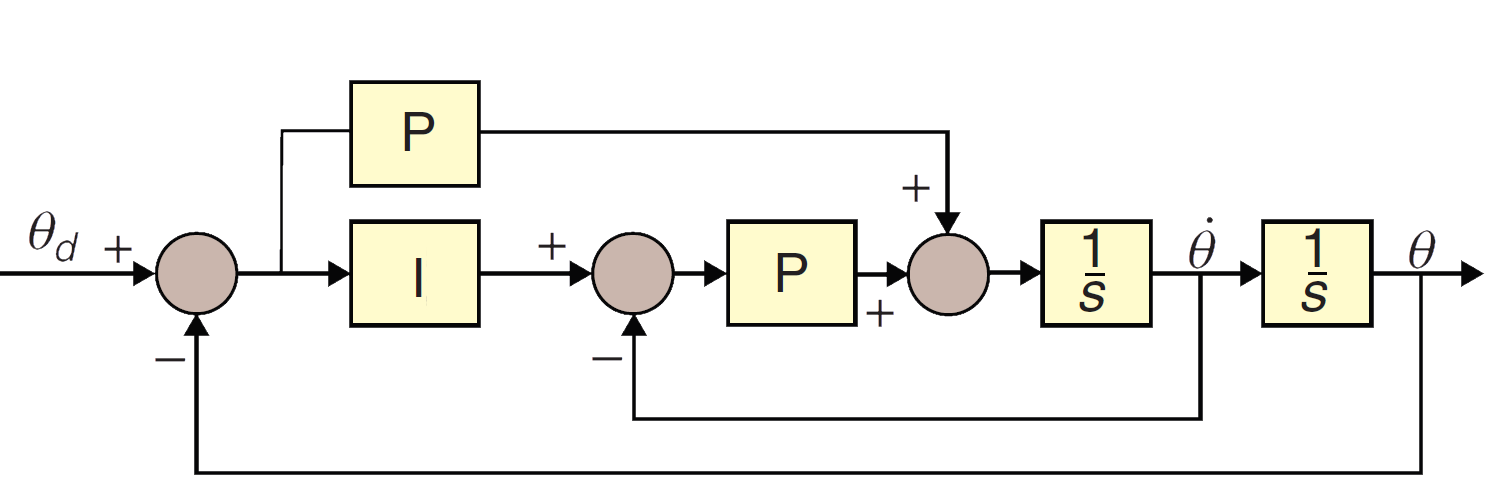
\includegraphics[width=0.8\textwidth]{figs/arducopter-pi}
\caption{ArduCopter PI Euler Angle Attitude Control loop}
\label{fig:arducopter-pi}
\end{figure}
Commercial flight controllers (Arducopter\cite{arducoptersite}, Openpilot\cite{openpilotsite}\footnote{\underline{NOTE:} OpenPilot's firmware branch is now maintained by LibrePilot} etc \ldots) for custom fabricated UAV platforms all apply their own structured attitude controllers and state estimation algorithms, based on onboard hardware sensor fusion. The article \emph{Build Your Own Quadrotor}\cite{buildyourownquad} summarizes the control structures implemented on a range of common flight controllers. The most popular of which, the Arducopter, implements a feed-forward PI compensation controller (Fig:\ref{fig:arducopter-pi}\footnote{Image sourced from \emph{Build your own Quadrotor}\cite{buildyourownquad}}).  PI, PD and PID controllers are all easy and effective independent control solutions for general attitude plants once the systems have been linearised. Table:\ref{tab:controllers} collectively lists the common attitude control blocks (not exclusively quadrotors UAVs but MAVs too) and which projects they've been implemented in, after which a critique on the more unique adaptations is given.
\begin{table}[h]
\centering
\begin{tabular}{ |c|l|l|c| }
\hline
Controller Type & Independent & Dependent & Total\\ \hline
PI & \cite{attitudecontrolproblem} & \cite{attitudecontrolproblem} & PI\\ \hline
PD & \cite{modelingquadcopter, tiltrihani} & \cite{fullquaternion,singleaxistilting} & PD\\ \hline
PID & \cite{optimizedpidquadcopter, attitudecontrolproblem, quaddynamics, tiltpropellercontrol, pidlqr} & \cite{attitudecontrolproblem, starmac, adaptivedisturbancecontrol} & PID\\ \hline
Lead & \cite{x4flyer, dynamicmodelling2009} & lead & lead\\ \hline
IBC & \cite{tpheonix, backsteppingquadcoptercontrol}\footnote{\cite{tpheonix} applied an IBC algorithm derived through Hurwitz polynomials, not lyupanov theorem.} & \cite{backsteppingquadcoptercontrol} & IBC\\ \hline
ABC & \multicolumn{2}{l|}{\cite{adaptivebackstep, nonlinearadaptive, 6dofbackstep, intelligentbackstep}} & ABC\\ \hline
LQR & \cite{pidlqr} & LQR & LQR\\ \hline
\end{tabular}
\caption{A Breakdown of common Attitude Controllers}
\label{tab:controllers}
\end{table}
\par
In a collection of papers, written by Bouabdallah et al \ldots (2003,2004,2007) arguably the most prolific early quadrotor authors, a range of different control implementations are derived and reviewed. Their last paper (2007)\cite{fullquadcoptercontrol} derived and pratically tested an Integral Backstepping attitude controller on an OS4 quadrotor. It builds on their research from an earlier paper (2003)\cite{pidlqr} wherein an analysis of PID vs LQR attitude controllers in the context of quadrotors is posed. LQR controllers aim to optimize the controller effort (that being $||\mathbb{U}||$ or the $L_2$ norm of the plant input) and although, in theory, solving the assocaited Ricatti cost function may produce an optimially stable and efficient control law it needs exact plant matching. In practice, direct plant identification is difficult to achieve for a quadcopter or any aerospace body for that matter. The resultant controller in \cite{pidlqr} achieved asymptotic stability but had poor steady state performance due to low fidelity of actuator dynamics and poor confidence inertial measurements.
\par
Adaptive Backstepping Control\cite{backstepping}(any of the examples in Table:\ref{tab:controllers}) expands on nominal IBC fundamentals by introducing an added estimated disturbance state term in the LCF used for the backstepping iteration. The caveat with this form of Backstepping approach is that, from the Lyupanov control theorem, a time derivative for the estimated disturbance (or an \emph{update law}) is needed. Disturbance approximation has been investigated thoroughly but, for a signal without any apriori information, some heuristic needs to be adopted with the approximation. In one example, \cite{nonlinearadaptive}, the authors implemented a statistical $proj(.)$ operator based technique. When used in adaptive control the projection operator \cite{outputfeedback}, $proj(.)$, ensures a derivative based estimator is bounded for adaptive regression approxmation \cite{nonlinearregression}.
\par
Although the control implementation isn't backstepping based, in \cite{adaptiveslidingmode}, a sliding mode controller was used to compensate for the disturbances in an Unmanned Submersible Vehicle atttiude plant. The underwater current disturbances are approximated using a fuzzy logic system, specifically a \emph{zero-order TSK} fuzzy controller. The TSK system has been proven to act in the same way as an Artificial Neural Network approximator\cite{zeroTSK}; where the TSK system is more comprehensible than the latter. Statistical analysis and investigation of approximators without a priori knowledge of a system are well beyond the scope of what this project hopes to achieve but are worth mentioning.
%====================================================
\subsubsection*{Single/Dual Axis Control \& Allocation}
%====================================================
The extra actuation introduced with single and dual axis articulation provides room for extra control goals to be achieved as the system actuation increases. Of the few papers published on tilting-axis quadrotors, PD (Nemati et al.[2014]\cite{singleaxistilting} and again in Gasco \& Rihani \cite{tiltgasco,tiltrihani}) and PID (Ryll et al.[2012,2013]\cite{tiltpropellercontrol,tiltpropellerflight}) are the norm for control blocks. For both of these systems there needs to be an allocation rule to distribute a commanded input amongst the actuator set. In \cite{allocation}, Johansen et al.[2012] describes the control allocation problem for a dynamic plant:
\begin{subequations} 
\raggedright
\begin{equation} \label{eq:3.1}
\dot{x}=f(x,t)+g(x,t)\tau
\end{equation}
\vspace{-20pt}
\begin{equation} \label{eq:3.2}
y=l(x,t)
\end{equation}
\end{subequations}
\\\emph{\color{Gray} Note in state space Equation:\ref{eq:3.1}, it's assumed the plant input, $\tau$, has a multiplicative relationship with the response, $g(x,t)\tau$.}
\\
with a state $x\in \mathbb{R}^n$ and $f(x,t)$ \& $g(x,t)$ being the plants' dynamic and input responses respectively. In set point tracking, the output is then \emph{tracking} the state $y = x$, and hence $y \in \mathbb{R}^n$. In an ideal well posed system the number of actuator inputs equals the number of controllable variable outputs; $dim(x)=dim(\tau)\in \mathbb{R}^n$. In the case where the input $\tau \in \mathbb{R}^m,m>n$ the problem is overactuated and a level of abstraction is needed; a virtual control input $\nu_d$ is designed by a control law $\nu_d=h(x_e,t)$ to effect dynamics. The objective is to then find a function that maps $\mathbb{R}^m \rightarrow \mathbb{R}^n$ for an actuator matrix $u \in \mathbb{U}^m$. 
\begin{subequations}
\begin{equation} \label{eq:3.3}
\dot{x}=f(x,t)+g(x,t)\nu_d,~\nu_d \in \mathbb{R}^n
\end{equation}
\vspace{-20pt}
\begin{equation}
\nu_d=B(x,t,u)\approx B(x,t)u, ~u\in \mathbb{U}
\end{equation}
\vspace{-20pt}
\begin{equation}
y=x
\end{equation}
\end{subequations}
$B(x,t,u)$ is the allocation rule and can, if the plant permits it, be abstracted to a multiplicative relationship $B(x,t)u$ such that; $B(x,t)\in\mathbb{R}^{n\times m}$. If the primary objective is setpoint tracking, then the control law will design $\nu_d$ which will achieve well that goal, the allocation rule then has to find $u$ for $\nu_d$:
\begin{equation}\label{eq:quadraticallocator}
\underset{u \in \mathbb{R}^m ,s \in \mathbb{R}^n}{min}\norm{Q_s} ~\text{subject to} ~\nu_c - h(x_e,t)=\nu_c-\nu_d=s, u \in \mathbb{U}
\end{equation}
Which ensures the commanded input $\nu_c$ tracks the control designed input $\nu_d$; $\nu_c\rightarrow\nu_d$. In an overactuated system it then follows that for an unique actuator solution (rather than a family solution set) to Eq:\ref{eq:quadraticallocator} a secondary objective function is needed, $J(x,t,u)$. Eq:\ref{eq:quadraticallocator} then becomes;
\begin{equation}
\underset{u \in \mathbb{R}^m ,s \in \mathbb{R}^n}{min}(\norm{Q_s}+J(x,t,u)) ~\text{subject to} ~\nu_c - h(x_e,t)=s, u \in \mathbb{U}
\end{equation}
\par
Over-actuation is not something often applied to quadrotors and as a result rather than providing a comprehensive literature review of associated papers here (which is mostly theoretical derivation), the contextual application and solutions to the above posed problems are expanded later in Section: \ref{subsec:control.allocation.allocators}. The only overactuated quadrotor (birotor dual-axis tilting makes the system critically actuated and so requires no allocation) literature which covers allocation of the given actuators is \cite{tiltgasco,tiltrihani}, where the authors apply a weighted pseudo inverse (sic Moore Penrose Inverse \cite{moorepenrose}) allocation rule.
%====================================================
\subsubsection*{Satellite Attitude Control}
%====================================================
Unconstrained attitude set-point tracking for 6-DOF bodies, quaternion based or otherwise, is a topic well covered in the field of satellite attitude control; \cite{axissymmetricspacecraft, satellitebackstepping,lpvbackstepping}. The \emph{status quo} for recent research is on non-linear adaptive attitude back-stepping control systems, wherein the adaptive update rule is the novel focus. Often plant uncertainty affects the inertia tensor of a satellite. In \cite{lpvbackstepping}, the authors Wang Jia, et al. [2010], proposed applying adaptive back-stepping to compensate for steady state (asymmetric) inertial estimation errors. Alternatively, in lieu of deliberating on an costly non-orbital prelaunch inertial measurements, \cite{inertiaestimation} developed an algorithm for estimating the inertia tensor based on single axis controlled perturbations.
\par
Satellite actuator sets tend to include additional redundant effectors, to ensure fault tollerance and reliability, and hence require control allocation. Seen in the paper \cite{satellitebackstepping}; the authors, Kristiansen et al. [2005], address the over-actuation with direct and well-matched inversion before applying quaternion based back-stepping for attitude control. 
\vspace{-10pt}
\begin{subequations}\label{eq:pseudoinv}
\begin{equation}\label{eq:pseudoinva}
u=B^{\dagger}({\tau_a}^{b}-D{\omega_{ib}}^b)
\end{equation}
\vspace{-20pt}
\begin{equation}\label{eq:pseudoinvb}
B^\dagger=B^T(BB^T)^{-1}
\end{equation}
\end{subequations}
Where $B$ is the control effectiveness matrix and $B^{\dagger}$ is such that $BB^{\dagger}=\mathbb{I}$. Specifically $B^{\dagger}$ is the general \emph{pseudo} inverse of $B$ (more on inversions in Sec:\ref{sec:control.allocation}). It's assumed there's a multiplicative relationship between the input, $u\in\mathbb{U}$, and the input effectiveness matrix. The controller designed actuator torque ${\tau_a}^b$ then dictates the input $u$ as in Eq:\ref{eq:pseudoinva}. Much like the over-actuation previously discussed W.R.T quadcopters; the pseudo inversion method of control distribution applies quadratic optimization to the allocation slack cost function, Eq:\ref{eq:quadraticallocator}. 